\documentclass[12pt]{article}%

\usepackage{fancyhdr}
\pagestyle{fancy}
\fancyhf{}
\fancyhead[R]{\thepage}

\usepackage{cmap}				
\usepackage{mathtext} 
\usepackage{listings}

\usepackage{biblatex}
\addbibresource{lib.bib}

\usepackage{euscript}
\usepackage{mathrsfs}

\usepackage[T2A]{fontenc}
\usepackage[utf8]{inputenc}
\usepackage[english,russian]{babel}
\usepackage{amsmath,amsfonts,amssymb,amsthm,mathtools}

\setlength\fboxsep{3pt}
\setlength\fboxrule{1pt}

% Работа с графикой и рисунками
\usepackage{graphicx} 
\usepackage{subcaption}

\usepackage{hyperref}
\usepackage[usenames,dvipsnames,svgnames,table,rgb]{xcolor}
\usepackage{wrapfig}
\hypersetup{				
    unicode=true,           
    pdftitle={Заголовок},   
    pdfsubject={Тема},      
    pdfkeywords={keyword1} {key2} {key3},
    colorlinks=true,
    linkcolor=black,
    citecolor=black,
    filecolor=magenta,
    urlcolor=cyan
}

% Работа с Python
\usepackage{minted}
\definecolor{LightGray}{gray}{0.98}

% Работа с enumerate
\usepackage{enumitem}

\newcommand*{\Title}{\begingroup
\centering 

\large {Федеральное автономное образовательное учреждение высшего образования}
\vspace*{\baselineskip}

\large {«Национальный исследовательский университет «Высшая школа экономики»»}
\vspace*{\baselineskip}

\vspace*{\baselineskip}
\large{\textbf{Отчет по лабораторной работе 7}}

\vspace{0.1cm}
\large{Численное решение стационарных и нестационарных задач теплопроводности}

\vspace{0.2cm}
\large{Вариант 10: задачи 10.1.10, 10.3.5, 10.4.10, 10.5.10, 10.6.10}

\vspace{1.5cm} 

\begin{flushright}
  \textbf{\normalsize Выполнил:}
  
  \vspace{0.3cm} 
  {\normalsize Студент группы БПМ-211}
  
  {\normalsize Ляхов Артём Андреевич}

\end{flushright}


\vspace{0.2cm}  
\begin{flushright}
  \textbf{\normalsize Преподаватель:} 

  \vspace{0.2cm}

 {\normalsize Брандышев Петр Евгеньевич}
 
\end{flushright}

\vfill
\date{}{Октябрь 2024 г.}


\endgroup\clearpage}

\begin{document}
\Title
\tableofcontents

\newpage
\section{Задача 10.1.10}
\subsection{Формулировка задачи}
Необходимо промоделировать стационарные процессы теплопроводности стержня в зависимости от входных данных задачи:
\begin{equation*}
\begin{cases}
    -\frac{d}{dx}\left(
        K(x) \frac{du}{dx}
    \right) = f \\
    u(a) = U_a,\ \ \ u(b) = U_b
\end{cases}
\end{equation*}

\begin{enumerate}
    \item Представить $K(x)$ в виде функции двух переменных $x$ и $c$: $K(x) = K(x, c)$, где $c$ - параметр
    \item При заданных в индивидуальном варианте $k(x)$ (набор 1) и $f(x)$ найти аналитическое решение задачи символьно.
    \item Изменяя значение параметра $c$ в коэффициенте теплопроводности, найти решения задачи для параметров 1-3 из таблицы.
    \item На одном чертеже построить найденные решения, сравнить полученные результаты.
    \item Аналогично п.2 найти аналитические решения для набора параметров 4. На одном чертеже построить решений для наборов 1 и 4. Сравнить полученные результаты.
    \item Изменяя граничные условия $U_a$, $U_b$, найти решения для наборов параметров 5-7. Изобразить их на одном чертеже. Сравнить полученные результаты.
\end{enumerate}

В соответствии с индивидуальным вариантом:

\begin{equation*}
k(x) = x,\ a = 0.1,\ b = 0.6,\ U_a = 1,\ U_b = 5
\end{equation*}

\newpage
\subsection{Результаты}
\begin{figure}[!h]
    \centering
    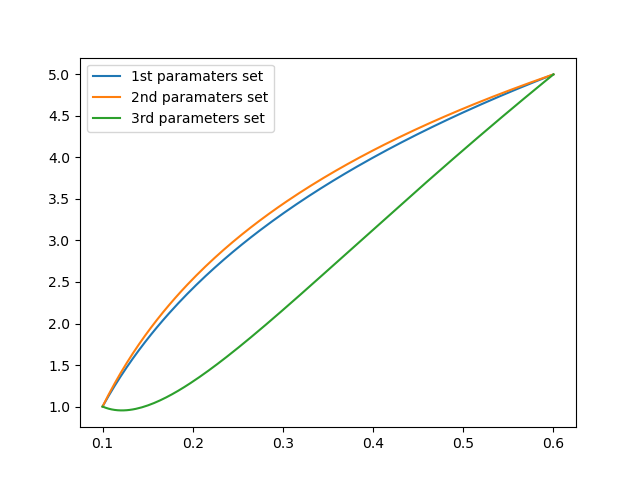
\includegraphics[width=0.65\textwidth]{sets1-3.png}
    \caption{Аналитические решения ДУ для наборов параметров 1-3.}
\end{figure}

\begin{figure}[!h]
    \centering
    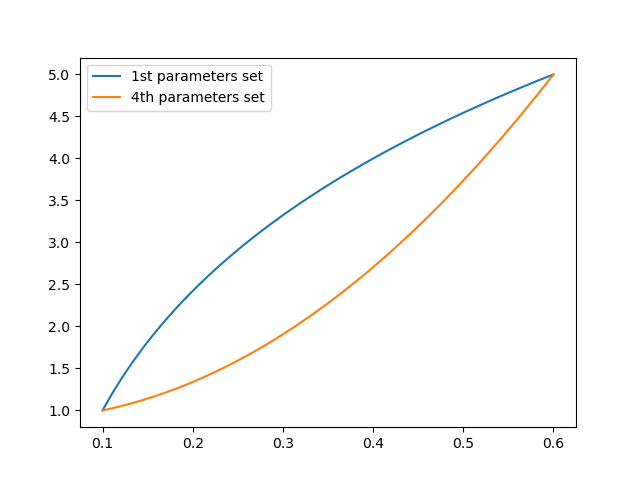
\includegraphics[width=0.65\textwidth]{sets14.png}
    \caption{Аналитические решения ДУ для наборов параметров 1 и 4.}
\end{figure}

\begin{figure}[!h]
    \centering
    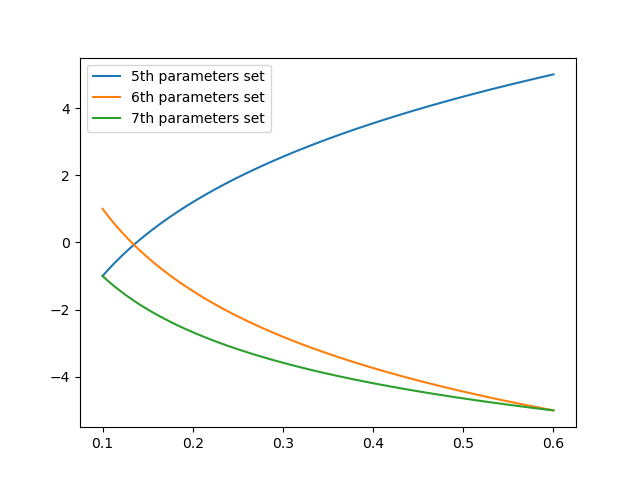
\includegraphics[width=0.65\textwidth]{sets5-7.png}
    \caption{Аналитические решения ДУ для наборов параметров 5-7.}
\end{figure}

\textbf{Вывод:} в нашем случае на поведение решения больше всего влияет изменение характера поведения функции $K(x)$ и изменение начальных условий.

\newpage

\section{Задача 10.3.5}
\subsection{Формулировка задачи}
Необходимо, используя метод конечных разностей, найти с точностью до $\varepsilon=0.1$ решение краевой задачи
\begin{equation*}
    \begin{cases}
        u''(x) - u'(x) + 2x^2 u(x) = x + 1 \\
        u(1.3) = 1 \\
        u(2.4) + u'(2.4) = 3.2
    \end{cases}
\end{equation*}
Изобразить решение на графике. Решение системы разностных уравнений найти, используя метод прогонки.

\subsection{Теоретический материал}
\subsubsection{Приближения второго порядка}
Обозначим за $u_i$ значение искомой функции $u(x)$ в узле $x_i$, за $h$ - длину шага сетки. 

Тогда для того, чтобы построить приближение значений функции $\{u_i\}^n_{i=0}$ необходимо составить систему разностных уравнений. Для этого можно воспользовать следующими аппроксимациями:
\begin{equation}\label{theor-d2-approx}
    u''_{i} \approx \frac{u_{i + 1} - 2 u_i + u_{i-1}}{h^2}
\end{equation}

\begin{equation}\label{theor-d1-approx}
    u'_i\approx \frac{u_{i+1} - u_{i-1}}{2h}    
\end{equation}

\begin{equation}\label{theor-d1-lower-bound}
    u'_{0} \approx \frac{-u_2 + 4u_1 - 3u_0}{2h}
\end{equation}

\begin{equation}\label{theor-d1-upper-bound}
    u'_{n} \approx \frac{3 u_n - 4u_{n-1} + u_{n-2}}{2h}
\end{equation}

Все приближения выше имеют второй порядок точности. Это значит, что разность между искомым значением и аппроксимацией равняется $O(h^2)$, при $h \rightarrow 0$.

\subsubsection{Метод прогонки}
Предположим, что нам необходимо решить систему линейных уравнений $Ax=b$, где $A$ - трёхдиагольная матрица, тогда по-другому эту систему можно записать в следующем виде:
\begin{equation}\label{theor-progonki-system}
    A_i x_{i - 1} + B_i x_{i} + C_i x_{i-1} = F_i
\end{equation}

Решить подобную систему можно, используя \textit{метод прогонки}. Этот метод основывается на предположении, что искомые неизвестные связаны рекуррентным соотношением:
\begin{equation}\label{theor-progonki-rec}
    x_{i} = \alpha_{i + 1} x_{i + 1} + \beta_{i + 1},\ \ 1 \le i \le n-1
\end{equation}
Подставив \ref{theor-progonki-rec} в уравнение \ref{theor-progonki-system}, мы получаем рекуррентные соотношения для $\alpha_{i}$ и $\beta_{i}$:
\begin{equation}\label{theor-progonki-coef1}
\begin{cases}
    \alpha_{i + 1} = \frac{-C_i}{A_i \alpha_i + B_i} \\
    \beta_{i + 1} = \frac{F_i - A_i \beta_i}{A_i \alpha_i + B_i}
\end{cases}
\end{equation}

\begin{equation}\label{theor-progonki-coef2}
\begin{cases}
    \alpha_2 = -C_1 / B_1 \\
    \beta_2 = F_1 / B_1
\end{cases}
\end{equation}

Таким образом, решение задачи методом прогонки состоит из двух частей. Первая, называемая \textit{прямой прогонкой} заключается в том, что, используя соотношения \ref{theor-progonki-coef1} и \ref{theor-progonki-coef2}, мы находим коэффициенты $\alpha_i$, $\beta_i$. Вторая часть, называемая \textit{обратной прогонкой}, состоит в нахождении $x_i$ при помощи соотношения \ref{theor-progonki-rec}.


\subsection{Решение задачи}
\subsubsection{Система разностных уравнений}
\begin{equation*}
    \frac{u_{i + 1} - 2 u_i + u_{i-1}}{h^2} -
    \frac{u_{i+1} - 
    u_{i-1}}{2h} + 2x_i^2 u_i = 
    x_i + 1\ \ \ 1 \le i \le n-1
\end{equation*}
Из начальных условий также получаем два уравнения:

\begin{equation*}
\begin{cases}
    u_0 = 1 \\
    u_n + \frac{3 u_n - 4u_{n-1} + u_{n-2}}{2h} = 3.2
\end{cases}
\end{equation*}

После преобразований и исключения переменной $u_{n-2}$ из уравнения для второго начального условия мы получаем итоговую систему разностных уравнений:
\begin{equation*}
\begin{cases}
    u_0 = 1 \\
    (2 - h) u_{i+1} + (-4 + 4x_i^2 h^2) u_i + (2 + h)u_{i-1} = 
    2h^2 (x_i + 1) \hspace{0.5cm} 1 \le i \le n \\
    (2h^2 + 8h + 4) u_n - 4(h + 1 + x_{n-1}^2 h^2) u_{n-1} = 
    6.4h(h + 2) - 2 h^2 (x_{n-1} + 1)
\end{cases}
\end{equation*}

Обратим внимание, что из первого уравнения получившейся системы мы сразу знаем $u_0$. В дальнейшем если мы будем воспринимать $u_0$ как известную константу, то мы можем заметить, что получившаяся система линейных уравнений относительно $u_1, \dots u_n$ имеет трёхдиагональную матрицу и может быть решена с помощью метода прогонки. 


% \newpage
\subsubsection{Результаты}
\begin{figure}[H]
    \centering
    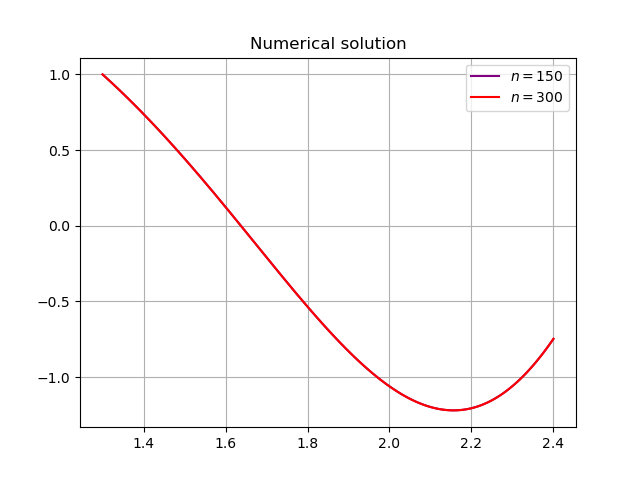
\includegraphics[width=0.8\textwidth]{solutions.png}
    \caption{Графики найденных решений для $n=150$ и $n=300$. Точность решения для $n=150$ оценивалась по правилу Рунге и составляла $1.1 \cdot 10^{-4}$.}
\end{figure}

\subsubsection{Код на Python}
\begin{minted}[
frame=single,
framesep=10pt,
framerule=0.1pt,
bgcolor=LightGray
]{python}
def tridiagonal_solver(l, m, u, r):
    """
    Solves a system of linear equations 
    with a tridiagonal matrix by the run-through method.

    :param l np.ndarray: the lower diagonal of matrix.
    :param: np.ndarray m: the main diagonal of matrix.
    :param: np.ndarray u: the upper diagonal of matrix.
    :param: np.ndarray r: the right size of system.

    :return np.ndarray: vector with solution of system
    """
    n = m.size       # l.size = u.size = n - 1
    a = np.zeros(n)
    b = np.zeros(n)

    a[0] = -u[0] / m[0]
    b[0] = r[0] / m[0]

    for i in range(1, n-1):
       a[i]=-u[i] / (l[i-1] * a[i-1] + m[i])
       b[i]=(r[i] - l[i-1] * b[i-1]) \
       /(l[i-1] * a[i-1] + m[i])

    X = np.zeros(n)
    b[n - 1]= (r[n - 1] - l[n - 2] * b[n - 2])\
    /(m[n - 1] + l[n - 2] * a[n - 2])
    X[n - 1] = b[n - 1]

    for i in range(n - 2, -1, -1):
        X[i] = a[i]*X[i+1] + b[i]
    return X
\end{minted}

\begin{minted}[
frame=single,
framesep=10pt,
framerule=0.1pt,
bgcolor=LightGray
]{python}
    def get_solution3(n):
    a = 1.3
    b = 2.4

    Ua = 1
    Ub = 3.2

    h = (b - a) / n
    x_arr = np.linspace(a, b, n + 1)


    lower = np.zeros(n - 1)
    main = np.zeros(n)
    upper = np.zeros(n - 1)
    b = np.zeros(n)

    
    for i in range(n):
        x = x_arr[i+1]
    
        if i == 0:
            main[i] = -4 + 4 * (x ** 2) * (h ** 2)
            upper[i] = 2 - h
            b[i] = 2 * (h ** 2) * (x + 1) - (2 + h) * Ua
    
        elif 0 < i and i < n-1:
            lower[i - 1] = 2 + h
            main[i] = -4 + 4 * (x ** 2) * (h ** 2)
            upper[i] = 2 - h
            b[i] = 2 * (h ** 2) * (x + 1)
        else:
            x_prev = x_arr[-2]

            lower[i - 1] = -4 * h - 4 - 4 * \
                (x_prev ** 2) * (h ** 2)
            main[i] = 2 * (h ** 2) + 8 * h + 4
            b[i] = 2 * h * Ub * (h + 2) - \
                2 * (h ** 2) * (x_prev + 1)


    y_arr = np.zeros(n + 1)
    y_arr[0] = Ua
    y_arr[1:] = tridiagonal_solver(lower, main, upper, b)

    return x_arr, y_arr

\end{minted}

\newpage
\section{Задача 10.4.10}
\subsection{Формулировка задачи}
Промоделировать стационарные теплопроводности стержня в зависимости в зависимости от входных данных задачи - переменного коэффициента теплопроводности $k(x)$ и плотности источников тепла $f(x)$:
\begin{equation*}
\begin{cases}
    -\frac{d}{dx}\left( k(x) \frac{du}{dx} \right) = f \\
    u(a) = U_a,\ \ \ u(b) = U_b
\end{cases}
\end{equation*}

Порядок решения задачи:
\begin{enumerate}
    \item Составить разностную схему второго порядка точности для решения указанной задачи.
    \item Взять исходные данные из задачи 10.1.10 ($a=0.1, \ b=0.6,\ U_a=1,\ U_b=5,\ k(x)=x,\ f(x)=\ln(x)$), шаг сетки положить равным $h = (b - a)/150$.
    \item Промоделировать процесс теплопроводности в зависимости от коэффициента $k(x)$. Сначала для случая, когда стержень состоит из двух материалов:
    \begin{equation*}
    \begin{cases}
        k_1,\ a \le x \le (b + a)/2 \\
        k_2,\ (b + a)/2 < x \le b
    \end{cases}
    \end{equation*}
    для ситуаций а)$k_1 \ll k_2$, б)$k_1 \gg k_2$ 
    
    Затем для случая, когда стержень состоит из трёх материалов:
    \begin{equation*}
    \begin{cases}
        k_1,\ a \le x \le a + (b - a)/3 \\
        k_2,\ a + (b - a)/3 < x \le a + 2(b - a)/3 \\
        k_3,\ a + 2(b - a)/3 < x \le b
    \end{cases}
    \end{equation*}
    для ситуаций а)$k_1 < k_2 < k_3$, б)$k_1 > k_2 > k_3$, в) $k_1 = k,\ k_2 = 10k, k_3 = k$, г)$k_1 = 100k,\ k_2 = k, k_3 = 100k$

    \item Промоделировать процесс теплопроводности в зависимости от правой части - функции $f(x)$, предполагая, что $f(x)$ - точечный источник тепла, то есть $f(x) = c \delta(x - x_0)$. Рассмотреть следующие варианты: а) точечный источник поставлен в середину отрезка $[a, b]$, б) два одинаковых источника поставлены в разные точки, симметричные относительно середины отрезка, в) два различных источника поставлены симметрично. г) предложить свой вариант расположения источников. 
\end{enumerate}


\subsection{Решение задачи}
\subsubsection{Разностная схема}
Запишем ДУ из системы в следующем виде:
\begin{equation*}
    -k'(x) u'(x) - k(x) u''(x) = f(x)
\end{equation*}
Теперь запишем систему разностных уравнений, используя аппроксимации второго порядка для $u'(x)$ и $u''(x)$:
\begin{equation*}
    -k'_i \frac{u_{i+1} - u_{i-1}}{2h} - 
    k_i \frac{u_{i+1} - 2u_i + u_{i-1}}{h^2} = f_i
\end{equation*}
После дополнительных преобразований и с учётом начальных условий система разностных уравнений будет иметь следующий вид:
\begin{equation*}
\begin{cases}
u_0 = U_a, \hspace{0.4cm} u_n = U_b \\ 
(-h k'_i - 2 k_i) u_{i+1} + 4 k_i u_i + (h k'_i - 2k_i) u_{i-1} = 2h^2 f_i\hspace{0.3cm} 1 \le i \le n-1 \\
\end{cases}
\end{equation*}

\subsubsection{Результаты}
\begin{figure}[H]
    \centering
    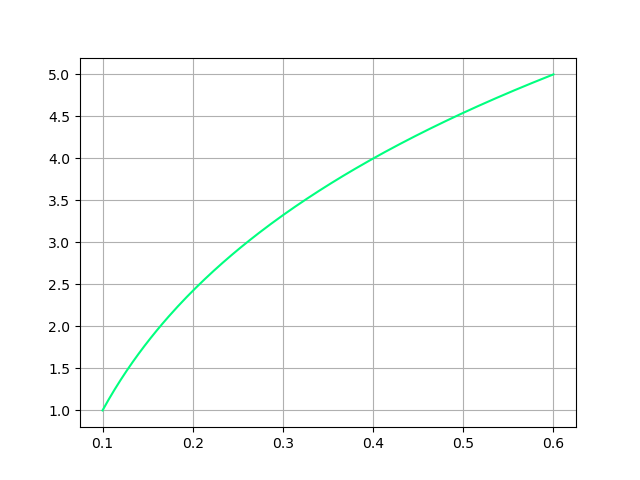
\includegraphics[width=0.65\textwidth]{task1.png}
    \caption{График функции $u(x)$ для первого набора параметров из задачи 10.1.10.}
\end{figure}

\begin{figure}[H]
\centering
\begin{subfigure}{0.49\textwidth}
    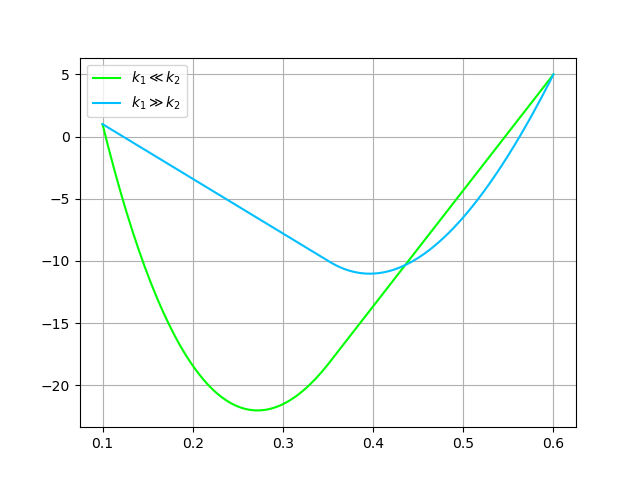
\includegraphics[width=\textwidth]{task21.png}
    \caption{Два материала}
\end{subfigure}
\hfill
\begin{subfigure}{0.49\textwidth}
    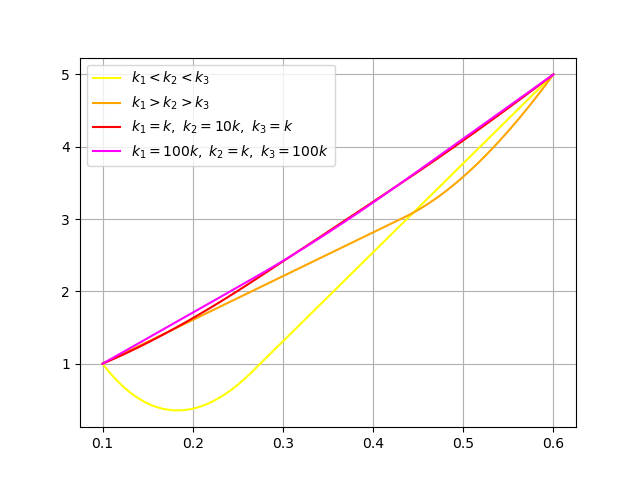
\includegraphics[width=\textwidth]{task22.png}
    \caption{Три материала}
\end{subfigure}
\caption{График функции $u(x)$ для случаев, когда стержень состоит из двух и трёх материалов. 
Для случая двух материалов брались значения:
а) $k_1 = 10^{-3},\ k_2 = 10^3$, 
б) $k_1 = 10^3,\ k_2=10^{-3}$. 
Для трёх материалов значения составляли: 
а) $k_1=10^{-2},\ k_2=150,\ k_3=10^4$
б) $k_1=10^{4},\ k_2=150,\ k_3=10^{-2}$
в-г) $k=0.1$.}
\end{figure}

\begin{figure}[H]
    \centering
    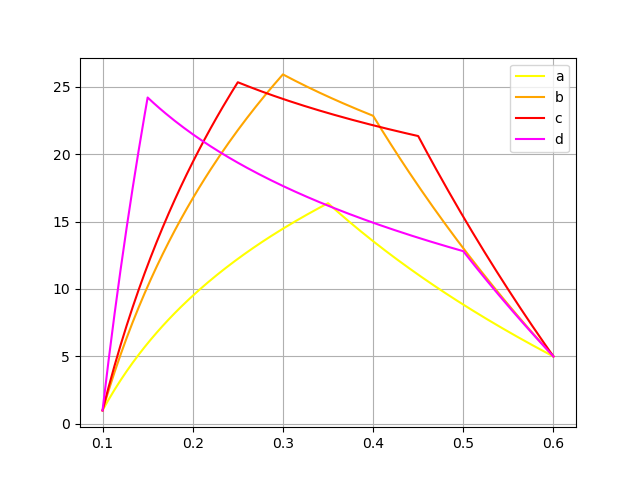
\includegraphics[width=0.65\textwidth]{task3.png}
    \caption{График функции $u(x)$ при моделировании с использованием точечного источника тепла. При моделировании использовалось $c=10^4$. Вариант d включал в себя расположение двух источников, первый из которых имел мощность $2c$ и находился на расстоянии $0.1 (b - a)$ от начала отрезка, второй имел мощность $c$ и находился на расстоянии $0.2 (b - a)$ от конца отрезка.  
    }
\end{figure}

\subsection{Код на Python}
\begin{minted}[
frame=single,
framesep=10pt,
framerule=0.1pt,
bgcolor=LightGray
]{python}
    def get_solution4(n, k_func, k_der_func, f_func, 
    a, b, Ua, Ub):
    h = (b - a) / n
    
    x_arr = np.linspace(a, b, n + 1)
    
    lower = np.zeros(n - 2)
    main = np.zeros(n - 1)
    upper = np.zeros(n - 2)
    b_arr = np.zeros(n - 1)

    x_arr = np.linspace(a, b, n + 1)
    
    for i in range(n-1):
        xi = x_arr[i+1]
        ki = k_func(xi)
        dki = k_der_func(xi)
        fi = f_func(xi)
    
        if i == 0:
            main[i] = 4 * ki
            upper[i] = -h * dki - 2 * ki
            b_arr[i] = 2 * (h ** 2) * fi - \
                Ua * (h * dki - 2 * ki)
    
        elif 0 < i and i < n-2:
            lower[i-1] = (h * dki - 2 * ki)
            main[i] = 4 * ki
            upper[i] = -h * dki - 2 * ki
            b_arr[i] = 2 * (h ** 2) * fi
        else:
            lower[i - 1] = (h * dki - 2 * ki)
            main[i] = 4 * ki
            b_arr[i] = 2 * (h ** 2) * fi -\
                Ub * (-h * dki - 2 * ki)

    y_arr = np.zeros(n + 1)
    y_arr[0] = Ua
    y_arr[-1] = Ub
    y_arr[1:-1] = tridiagonal_solver(
        lower, main, upper, b_arr
    )
    return x_arr, y_arr
\end{minted}




\newpage
\section{Задача 10.5.10}
\subsection{Формулировка задачи}
Методом конечных разностей найти приближённое решение краевой задачи
\begin{equation*}
\begin{cases}
    -(k(x) u'(x))' + q(x)u(x) = f(x),\ \ x \in (a, b) \\
    -k(a)u'(a) + 0.5 u(a) = 0 \\
    k(b)u'(b) + 0.5 u(b) = 0,
\end{cases}
\end{equation*}
с тремя верными значащими цифрами. Решение системы разностных уравнений найти, использую метод прогонки.

Согласно индивидуальному варианту:
\begin{equation*}
k(x) = \begin{cases}
1.8,\ \ a < x < c \\
0.6,\ \ c < x < b
\end{cases}
\end{equation*}

\begin{equation*}
q(x) = \begin{cases}
6.5,\ \ a < x < c\\
7.8,\ \ c < x < b
\end{cases}
\end{equation*}

\begin{equation*}
f(x) = 8x (2.5 - x),\ \ a=0,\ b=2,\ c=1.125
\end{equation*}

\subsection{Решение задачи}
\subsubsection{Разностная схема}
Перепишем ДУ в другом виде:
\begin{equation*}
    -k'(x) u'(x) - k(x) u''(x) + q(x)u(x) = f(x)
\end{equation*}

Использовав аппроксимации второго порядка \ref{theor-d2-approx} и \ref{theor-d1-approx}, получаем систему разностных уравнений:
\begin{equation*}
    -k'_i \frac{u_{i+1} - u_{i-1}}{2h} - 
    k_i \frac{u_{i+1} - 2u_i + u_{i-1}}{h^2} + q_i u_i = f_i,\ \
    i \in \{1,\dots, n-1\}
\end{equation*}
Кроме того дополнительно подставим оценки \ref{theor-d1-lower-bound} и \ref{theor-d1-upper-bound} в начальные условия задачи, у нас выйдет ещё два уравнения:
\begin{equation*}
\begin{cases}
    -k_0 \frac{-u_2 + 4u_1 - 3u_0}{2h} + \frac{1}{2} u_0 = 0 \\
    -k_n \frac{3 u_n - 4u_{n-1} + u_{n-2}}{2h} + \frac{1}{2} u_n = 0
\end{cases}
\end{equation*}
После несложных преобразований учёта того, что в нашей задаче $k'(x) = 0$, и исключения $u_2$ и $u_{n-2}$ из первого и второго уравнения выше соответственно, получаем итоговую систему разностных уравнений:
\begin{equation*}
\begin{cases}
(-2 k_1 k_0 + h^2 k_0 q_1)u_1 + (2 k_0 k_1 + k_1 h)u_0 = k_0 f_1 h^2 \\
-k_i u_{i+1} + (2k_i + h^2 q_i) u_i - k_i u_{i-1} = f_i h^2,\ \ i \in \{1, \dots, n-1 \}\\
(2 k_n k_{n-1} + h k_{n-1})u_n + (-2k_n k_{n-1} + k_n h^2 q_{n-1})u_{n-1} = k_n f_{n-1} h^2
\end{cases}
\end{equation*}
Полученная система линейных уравнений относительно $u_0, \dots u_n$ имеет трёхдиагональную матрицу и может быть решена с помощью метода прогонки.

\subsubsection{Результаты}
\begin{figure}[H]
    \centering
    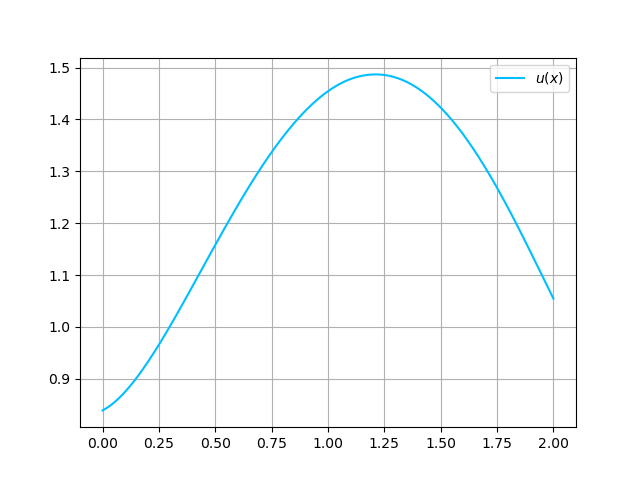
\includegraphics[width=0.75\textwidth]{problem5.png}
    \caption{Приближённое решение $u(x)$. В качестве $n$ бралось значение $n=300$. Оценка погрешности осуществлялась по правилу Рунге и составляет $7\cdot 10^{-4}$.}
\end{figure}

\newpage
\section{Задача 10.6.10}
\subsection{Формулировка задачи}
Промоделировать нестационарные процессы теплопроводности в зависимости от входных данных задачи - коэффициента теплопроводности $k(x)$ и начальной температуры $\phi(x)$:
\begin{equation*}
\begin{cases}
\frac{\partial{u}}{\partial{t}} =
\frac{\partial}{\partial{x}} \left(
k(x) \frac{\partial{u}}{\partial{x}}
\right) + f(x) (1 - e^{-t}),\ \ \ \ 0 < x < l,\ \ \ \ 0 < t < T \\
u(0, t) = UA, \ \ \ u(l, t) = UB, \ \ \ \ 0 \le t \le T \\
u(x, 0) = \phi(x), \ \ \ \ 0 \le x \le l
\end{cases}
\end{equation*}
Порядок решения:
\begin{enumerate}
    \item Найти приближённое решение задачи с шагами $\tau = 0.05$ и $h=0.1$, используя явную разностную схему. Построить графики решений при значениях $t = 0.5 \tau$, $t = 10 \tau$, $t = 20 \tau$.
    \item Используя результаты задачи 10.1, экспериментально определить момент времени $t$, при котором происходит установление процесса.
    \item Произвести анимацию процесса установления.
    \item Исследовать, как влияет начальная температура на процесс установления, взяв другие функции $\phi(x)$, согласованные с начальными условиями.
\end{enumerate}
Согласно индивидуальному варианту:
\begin{equation*}
k(x) = x,\hspace{0.5cm} f(x) = \ln(x),\hspace{0.5cm} \phi(x) = \frac{UB - UA}{b - a}(x - a) + UA
\end{equation*}
\begin{equation*}
    a = 0.1,\ UA = 1,\ b = 0.6,\ UB = 5
\end{equation*}

\subsection{Теоретический материал}
\subsubsection{Явные схемы}
Явные схемы - это численные методы, в которых для нахождения приближённого решения в $j+1$ момент времени используется только информация о приближённом решении в $j$ момент времени. Подобный подход позволяет в явном виде выписать значения $\{u_i^{j+1}\}^n_{i=0}$.

Явные схемы очень просты с точки зрения реализации, но при этом в большинстве случаев являются условно устойчивыми, что накладывает существенные ограничения на длину временного шага $\tau$.


\subsubsection{Неявные схемы}
Неявные схемы — это численные методы, где значения функции на следующем временном шаге зависят от неизвестных значений в текущем шаге. В большинстве случае, использование подобного подхода требует на каждом временном шаге решать систему линейных уравнений.

Неявные схемы являются более сложными с точки зрения реализации, по сравнению с явными схемы. Но при этом в большинстве задач неявные схемы обладают безусловной устойчивостью, что позволяет выбирать большие значения временного шага $\tau$ и делает процесс построения решения быстрым.

\subsection{Решение задачи}
Прежде, чем решать задачу, введём обозначение. $g(x, t) = f(x) (1 - e^{-t})$, а также раскроем уравнение в частных производных:
\begin{equation*}
    \frac{\partial{u}}{\partial{t}} = k(x) \frac{\partial^2{u}}{\partial{x}^2} + k'(x) \frac{\partial{u}}{\partial{x}} + g(x, t)
\end{equation*}

\subsubsection{Явная разностная схема}
Запишем конечные разности для решаемого дифференциального решения с использованием левой разности первого порядка для оценки $u'_t$:
\begin{equation*}
    \frac{u_i^{j+1} - u_i^{j}}{\Delta t} = 
    k_i \frac{u^j_{i+1} - 2u^j_i + u^j_{i-1}}{h^2} +
    k'_i \frac{u^j_{i+1} - u^j_{i-1}}{2h} + g^j_i
\end{equation*}

Выразим из этого равенства величину $u^{j+1}_i$:
\begin{equation*}
u^{j+1}_{i} = 
\Delta t \left( \frac{k'_i}{2h} + \frac{k_i}{h^2} \right) u^{j}_{i+1} + 
\left( 1 - \frac{2 \Delta t k_i}{h^2} \right) u^{j}_{i} + 
\Delta t \left( -\frac{k'_i}{2h} + \frac{k_i}{h^2} \right) u^{j}_{i-1} + 
\Delta t g^j_{i}
\end{equation*}

\subsubsection{Неявная разностная схема}
Для решаемого нами дифференциального уравнения запишем конечные разности, где $u'_t$ будем оценивать правой разностью:
\begin{equation*}
    \frac{u_i^{j+1} - u_i^{j}}{\Delta t} = 
    k_i \frac{u^{j+1}_{i+1} - 2u^{j+1}_i + u^{j+1}_{i-1}}{h^2} +
    k'_i \frac{u^{j+1}_{i+1} - u^{j+1}_{i-1}}{2h} + g^{j+1}_i
\end{equation*}

В данном случае мы уже не можем явно выразить $u^{j+1}_i$, однако мы можем составить систему линейных уравнений с трёхдиагональной матрицей, которую в будущем мы сможем решить с помощью метод прогонки:
\begin{equation*}
\Delta t \left( \frac{k'_i}{2h} + \frac{k_i}{h^2} \right) u_{i+1}^{j+1} +
\left( - 1 - \frac{2 \Delta t k_i}{h^2} \right) u_{i}^{j+1} + 
\Delta t \left( \frac{k_i}{h^2} - \frac{k'_i}{2h} \right) u_{i-1}^{j+1} =
-u_i^j - \Delta t g_i^{j+1}
\end{equation*}

\subsubsection{Результаты}
\begin{figure}[H]
    \centering
    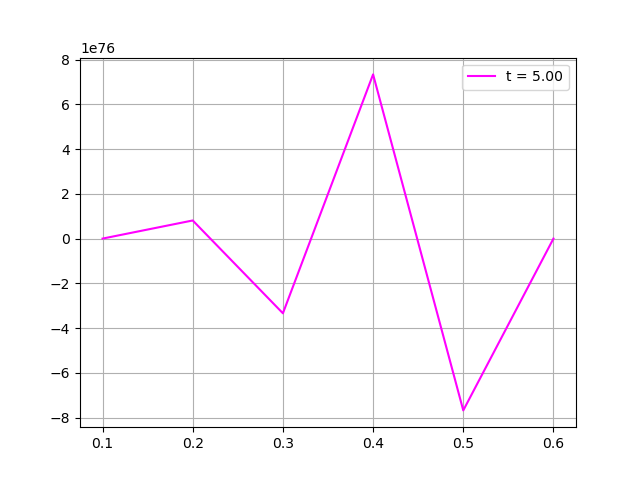
\includegraphics[width=0.65\textwidth]{explicit-failure.png}
    \caption{График $u(x)$ в момент времени $t=5$. Разностная схема - явная. Начальная температура - $\phi(x)$. Параметры сетки: $\Delta t = \tau = 0.05$, $h=0.1$.}
\end{figure}

Как мы можем наблюдать, при использовании параметров $\Delta t = \tau = 0.05$ и $h=0.1$ из условия задачи явная разностная схема разошлась. 

Эксперименты по подбору параметра $\Delta t$ показали, что при $\Delta t=0.01$ схема сходится. Анализ анимации процесса показал, что при $T=0.2$ происходит установление процесса.

\begin{figure}[H]
    \centering
    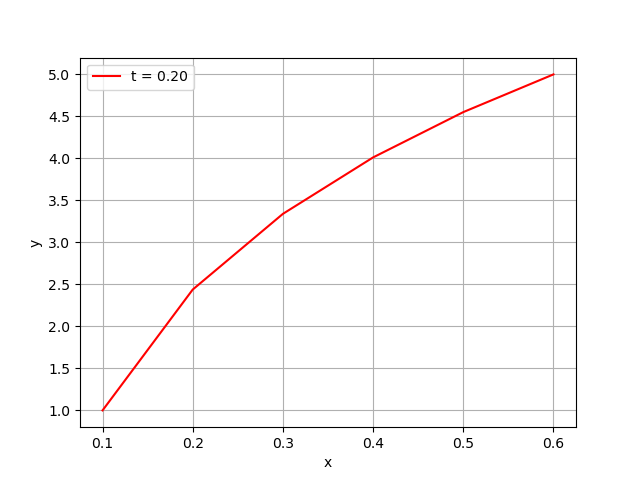
\includegraphics[width=0.65\textwidth]{explicit-stationarity.png}
    \caption{График решения в момент $t=0.2$. Разностная схема - явная. Начальная температура - $\phi(x)$. Параметры сетки: $\Delta t = 0.01$, $h=0.1$.}
\end{figure}


Дальнейший анализ изменения решения со временем будем производить, использую неявную схему. Это позволит ускорить процесс нахождение решения.


\begin{figure}[H]
\centering
\begin{subfigure}{0.32\textwidth}
    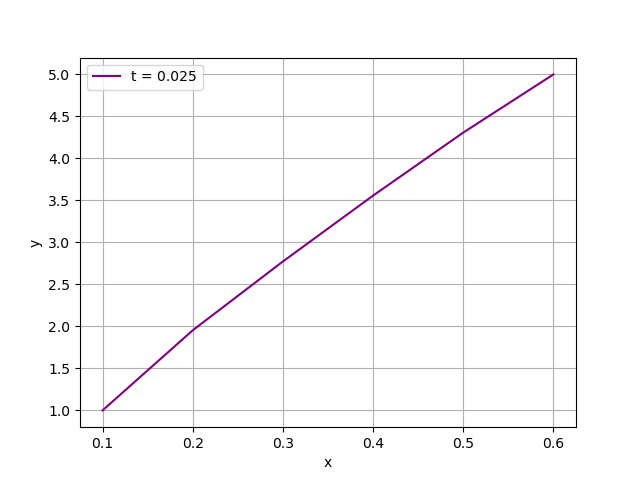
\includegraphics[width=\textwidth]{implicit-time0.025.png}
    \caption{$t = 0.5 \tau$}
\end{subfigure}
\hfill
\begin{subfigure}{0.32\textwidth}
    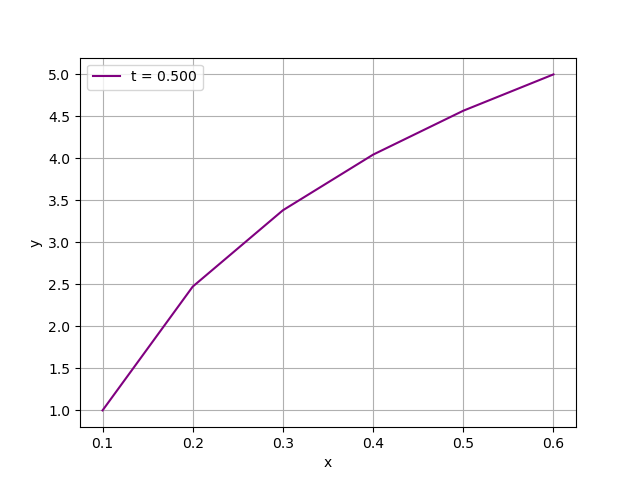
\includegraphics[width=\textwidth]{implicit-time0.500.png}
    \caption{$t = 10 \tau$}
\end{subfigure}
\hfill
\begin{subfigure}{0.32\textwidth}
    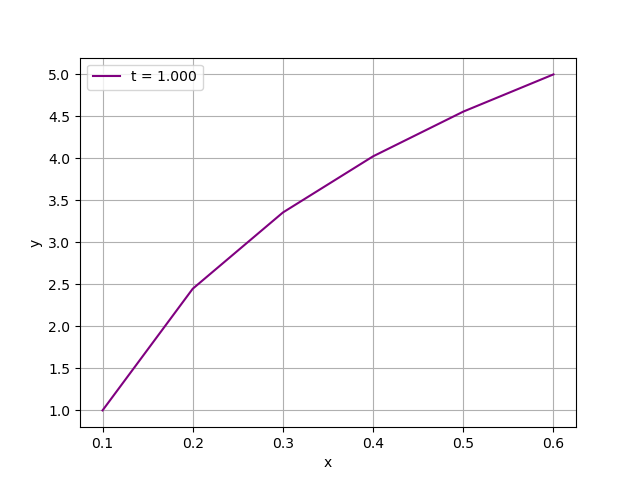
\includegraphics[width=\textwidth]{implicit-time1.000.png}
    \caption{$t = 20 \tau$}
\end{subfigure}
\caption{Графики решений в моменты $t = 0.5 \tau$, $t = 10 \tau$, $t = 20 \tau$. Разностная схема - неявная. Начальная температура - $\phi(x)$. Параметры сетки: $\Delta t = \tau / 2 = 0.025$, $h=0.1$.}
\end{figure}

Построим численное решение ещё для двух начальных температур. Для того, чтобы быть согласованной с начальными условиями $\hat{\phi}(x)$ должна удовлетворять:
\begin{equation*}
\begin{cases}
\hat{\phi}(a) = Ua \\
\hat{\phi}(b) = Ub
\end{cases}
\end{equation*}

В качестве второй функции-начальной температуры возьмём кусочно-постоянную функцию $\phi_2(x)$:
\begin{equation*}
\phi_2(x) = 
\begin{cases}
    Ua,\ a \le x \le (b + a)/2 \\
    Ub,\ (b + a)/2 < x \le b
\end{cases}
\end{equation*}

\begin{figure}[H]
\centering
\begin{subfigure}{0.32\textwidth}
    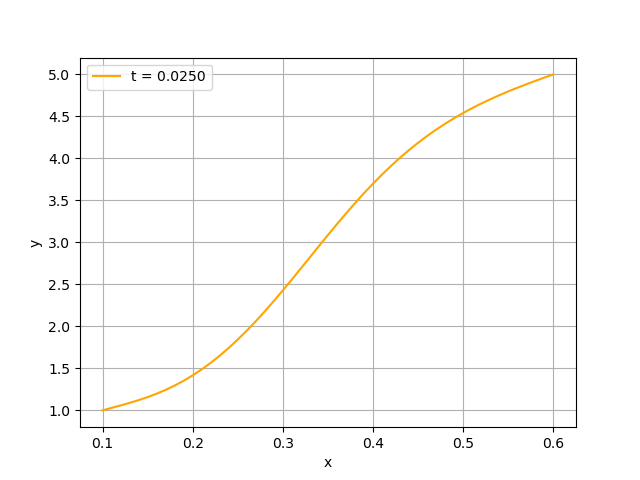
\includegraphics[width=\textwidth]{implicit-phi2-time-0.0250.png}
    \caption{$t = 0.5 \tau$}
\end{subfigure}
\hfill
\begin{subfigure}{0.32\textwidth}
    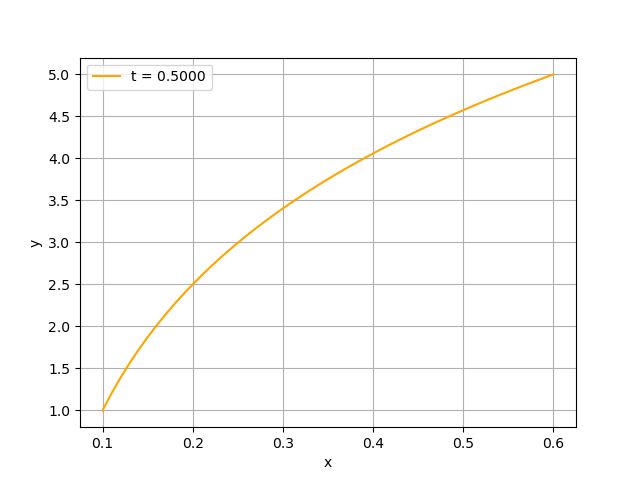
\includegraphics[width=\textwidth]{implicit-phi2-time-0.5000.png}
    \caption{$t = 10 \tau$}
\end{subfigure}
\hfill
\begin{subfigure}{0.32\textwidth}
    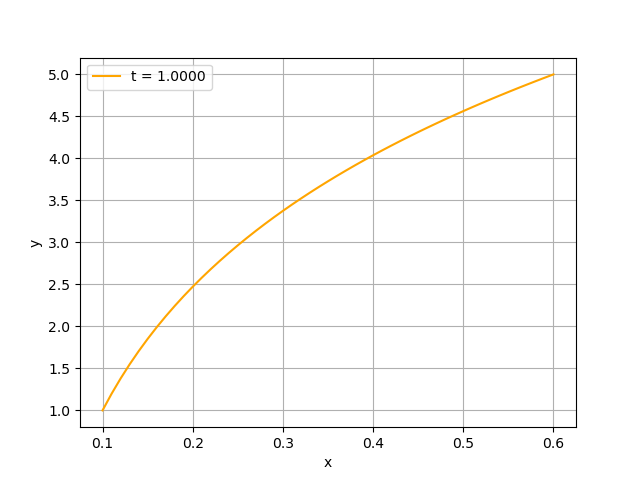
\includegraphics[width=\textwidth]{implicit-phi2-time-1.0000.png}
    \caption{$t = 20 \tau$}
\end{subfigure}
\caption{Графики $u(x, t)$ в моменты $t = 0.5 \tau$, $t = 10 \tau$, $t = 20 \tau$. Разностная схема - неявная. Начальная температура - $\phi_2(x)$. Параметры сетки: $\Delta t = \tau / 10 = 0.005$, $h=0.01$.}
\end{figure}

В качестве третьей функции-начальной температуры возьмём функцию, моделирующую два источника тепла, первый из которых находится в начале отрезка и имеет мощность $Ua$, второй - в конце отрезка и имеет мощность $Ub$:

\begin{equation*}
\phi_3(x) = U_a \cdot \delta (x - a) + U_b \cdot \delta (x - b)
\end{equation*}

\begin{figure}[H]
\centering
\begin{subfigure}{0.32\textwidth}
    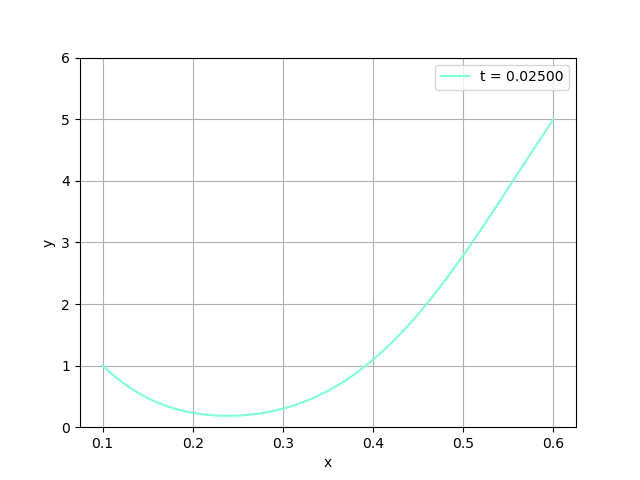
\includegraphics[width=\textwidth]{implicit-phi3-time-0.02500.png}
    \caption{$t = 0.5 \tau$}
\end{subfigure}
\hfill
\begin{subfigure}{0.32\textwidth}
    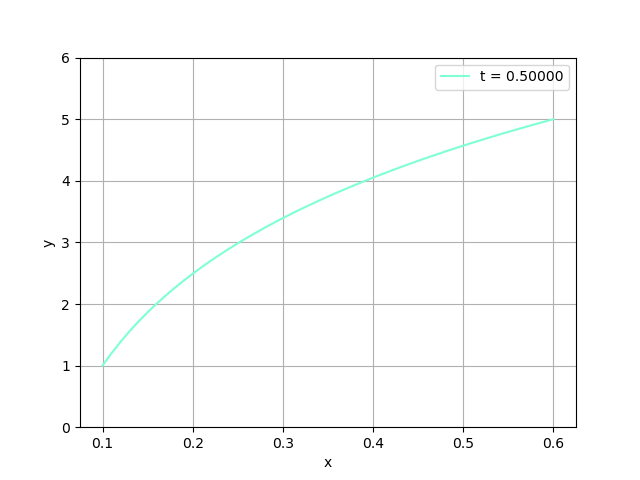
\includegraphics[width=\textwidth]{implicit-phi3-time-0.50000.png}
    \caption{$t = 10 \tau$}
\end{subfigure}
\hfill
\begin{subfigure}{0.32\textwidth}
    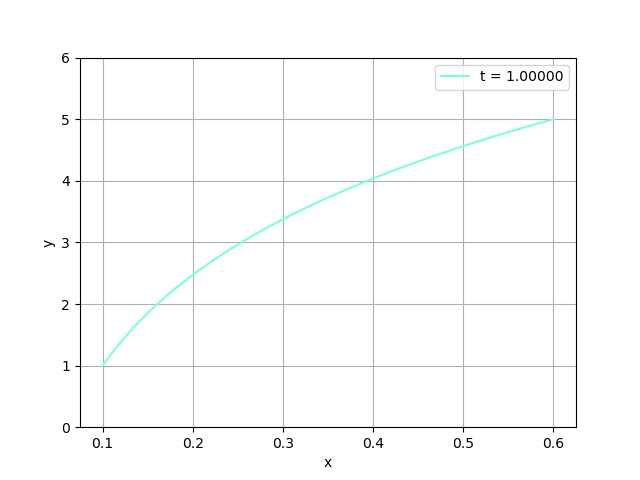
\includegraphics[width=\textwidth]{implicit-phi3-time-1.00000.png}
    \caption{$t = 20 \tau$}
\end{subfigure}
\caption{Графики $u(x, t)$ в моменты $t = 0.5 \tau$, $t = 10 \tau$, $t = 20 \tau$. Разностная схема - неявная. Начальная температура - $\phi_3(x)$. Параметры сетки: $\Delta t = \tau / 20 = 0.0025$, $h=0.01$.}
\end{figure}

Как мы можем для всех трёх начальных температур к моменту времени $T=0.2$ происходит установление одного и того же процесса.

\subsection{Анимации процессов}
Анимации процессов для начальных температур $\phi_1(x)$, $\phi_2(x)$ и $\phi_3(x)$ можно найти в zip-архиве Animations.zip, прикреплённом вместе с данным отчётом.

\subsection{Код на Python}
\begin{minted}[
frame=single,
framesep=10pt,
framerule=0.1pt,
bgcolor=LightGray
]{python}
class ExplicitNPDESolution:
    """
    Represents numerical solution of PDE 
    using explicit scheme
    """
    def __init__(self, k_func, k_der_func, g_func, 
    a, b, ua, ub, phi_func, tau, h):
        self.n = int((b - a) / h)
        self.time = 0
        self.tau = tau
        self.h = h
        self.bounds = (a, b)
        self.bc = (ua, ub)

        self.x_list = np.linspace(a, b, self.n + 1)

        self.ki_list = np.array(
            [k_func(x) for x in self.x_list]
        )
        self.dki_list = np.array(
            [k_der_func(x) for x in self.x_list]
        )
        self.y_list = np.array(
            [phi_func(x) for x in self.x_list]
        )

        self.g_function = g_func

    def get_solution(self, return_time=False):
        if return_time:
            return self.x_list, self.y_list, self.time
        return self.x_list, self.y_list

        def update(self):
        time = self.time
        ua, ub = self.bc
        tau, h = self.tau, self.h

        y_now = self.y_list
        y_next = np.zeros_like(self.y_list)
        y_next[0], y_next[-1] = ua, ub

        dki = self.dki_list
        ki = self.ki_list
        gi = np.array(
            [self.g_function(x, time) for x in self.x_list]
        )
        
        ai = tau * (dki[1:-1] / (2 * h) + ki[1:-1] / \
                (h ** 2))
        bi = (1 - (2 * tau * ki[1:-1]) / (h ** 2))
        ci = tau * (- dki[1:-1] / (2 * h) + ki[1:-1] / \
                (h ** 2))
        di = tau * gi[1:-1]

        y_next[1:-1] = ai * y_now[2:] + bi * y_now[1:-1] + \
                ci * y_now[:-2] + di
        
        self.time += self.tau
        self.y_list = y_next
\end{minted}

\begin{minted}[
frame=single,
framesep=10pt,
framerule=0.1pt,
bgcolor=LightGray
]{python}
class ImplicitNPDESolution:
    """
    Represents numerical solution of PDE 
    using implicit scheme
    """
    def __init__(self, k_func, k_der_func, g_func, 
    a, b, ua, ub, phi_func, tau, h):
        self.n = int((b - a) / h)
        self.time = 0
        self.tau = tau
        self.h = h
        self.bounds = (a, b)
        self.bc = (ua, ub)

        self.x_list = np.linspace(a, b, self.n + 1)

        self.ki_list = np.array(
            [k_func(x) for x in self.x_list]
        )
        self.dki_list = np.array(
            [k_der_func(x) for x in self.x_list]
        )
        self.y_list = np.array(
            [phi_func(x) for x in self.x_list]
        )

        self.g_function = g_func

    def get_solution(self, return_time=False):
        if return_time:
            return self.x_list, self.y_list, self.time
        return self.x_list, self.y_list

    def update(self):
        time = self.time
        ua, ub = self.bc
        tau, h = self.tau, self.h

        y_next = np.zeros_like(self.y_list)
        y_next[0], y_next[-1] = ua, ub

        upper = np.empty(0)
        lower = np.empty(0)
        main = np.empty(0)
        vector = np.empty(0)

        for i in range(1, self.n):
            xi = self.x_list[i]
            ki = self.ki_list[i]
            dki = self.dki_list[i]
            ui = self.y_list[i]
            gi = self.g_function(xi, time + tau)

            ai = tau * (dki / (2 * h) + ki / (h ** 2))
            bi = -1 - (2 * tau * ki) / (h ** 2)
            ci = tau * (ki / (h ** 2) - dki / (2 * h))
            di = -ui - tau * gi

            if i == 1:
                upper = np.append(upper, ai)
                main = np.append(main, bi)
                vector = np.append(
                    vector, di - ci * y_next[0]
                )
            elif i < self.n - 1:
                upper = np.append(upper, ai)
                main = np.append(main, bi)
                lower = np.append(lower, ci)
                vector = np.append(vector, di)
            elif i == self.n - 1:
                main = np.append(main, bi)
                lower = np.append(lower, ci)
                vector = np.append(
                    vector, di - ai * y_next[-1]
                )

        y_next[1:-1] = tridiagonal_solver(
            lower, main, upper, vector
        )
        
        self.y_list = y_next
        self.time += self.tau          
\end{minted}
\end{document}